% !Mode:: "TeX:UTF-8"
\chapter{系统需求分析与总体设计}

\section{系统功能需求分析}

根据第一章对DL框架Fuzzing产物管理问题的分析，
本系统围绕测试产物的管理和分析来进行数据处理。
进入系统的数据主要来自Fuzzing工具生成的测试脚本、执行日志等；
经过解析、向量化和统计分析之后，
系统向开发者提供数据管理界面和分析结果。
CEI评分、故障关联分析结果、辅助诊断报告和候选补盲结果等也会在分析页面中展示。
具体的功能性需求如表\ref{tab:function_requirements}所示。

\begin{table}[htbp]
\centering
\caption{系统功能需求分析表}
\label{tab:function_requirements}
\footnotesize
\renewcommand{\arraystretch}{1.15}
\begin{tabularx}{\textwidth}{>{\raggedright\arraybackslash}p{0.8cm}>{\raggedright\arraybackslash}p{2.0cm}>{\raggedright\arraybackslash}p{2.6cm}>{\raggedright\arraybackslash}p{2.7cm}>{\raggedright\arraybackslash}X}
\toprule
编号 & 功能需求 & 输入 & 输出 & 补充说明 \\
\midrule
FR-1 & 测试数据接入与特征提取 & 测试脚本、日志文件、算子拓扑结构 & 结构化元数据、日志向量、结构向量 & 为检索、统计和后续分析提供基础数据。 \\
FR-2 & AI智能分析助手 & 自然语言问题、错误描述、历史用例库 & 相似历史用例、辅助诊断报告 & 帮助开发者理解当前崩溃与历史样本之间的关系。 \\
FR-3 & 用例详情故障定位 & 单条用例日志、错误类型、计算图拓扑 & 候选算子节点位置、初步分析结果 & 用于在用例详情中缩小错误位置排查范围。 \\
FR-4 & 测试集多样性监测 & 测试用例向量、执行状态、筛选条件 & PCA二维投影结果、分布展示数据 & 用于观察样本是否集中在少数算子组合附近。 \\
FR-5 & 测试效能评估与低价值数据清退 & 覆盖贡献、执行成本、测试用例元数据 & CEI评分、低收益用例标记、清退结果 & 为冗余用例识别和数据清退提供依据。 \\
FR-6 & 故障关联分析 & 召回样例、成功样本、崩溃样本参数 & 候选边界条件、参数差分、相关样例 & 用于分析参数组合差异与崩溃现象之间的关联。 \\
FR-7 & 覆盖分析与算子缺口补盲 & 覆盖数据、算子组合关系、覆盖缺口 & 覆盖不足算子衔接、候选补盲测试脚本 & 将覆盖缺口转化为后续测试输入的候选数据。 \\
\bottomrule
\end{tabularx}
\end{table}

\section{系统总体架构设计}

本系统采用分层架构，
按照职责划分，系统从下到上分为数据层、算法处理层、服务调度层和应用层四部分，
整体结构如图\ref{fig:system_architecture}所示。
这种划分使界面展示、业务请求、算法计算和数据管理分别由不同层次承担，
可以减少不同实现细节之间的耦合。

\begin{figure}[!htbp]
\centering
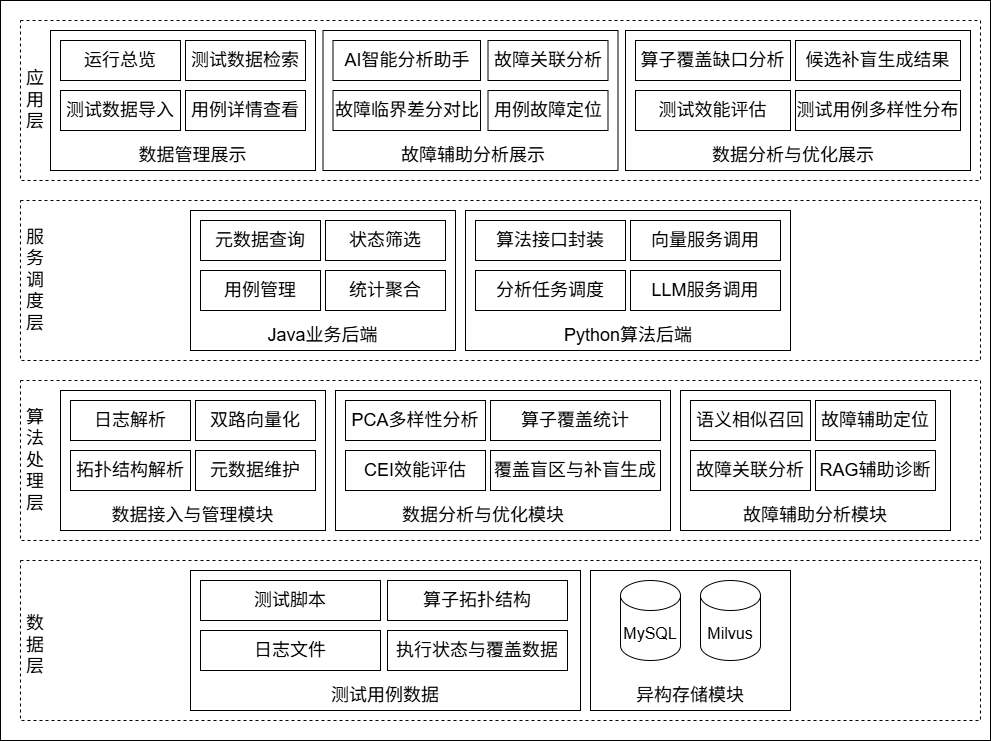
\includegraphics[width=0.85\textwidth]{figure/system_arc.png}
\caption{系统总体架构图}
\label{fig:system_architecture}
\end{figure}

数据层保存系统运行所需的数据资源，
分为测试用例数据和异构存储模块两部分。
测试用例数据由测试脚本、日志文件、算子拓扑结构、执行状态与覆盖数据等组成。
异构存储模块由MySQL和Milvus共同承担，
其中MySQL保存结构化元数据、状态字段和覆盖统计结果，
Milvus保存日志向量和结构向量，
两者共同实现条件查询、相似用例召回，以便后续分析。

算法处理层提供系统分析能力，
按照数据处理方向划分为数据接入与管理模块、数据分析与优化模块和故障辅助分析模块。
数据接入与管理模块负责日志解析、拓扑结构解析、双路向量化和元数据维护；
数据分析与优化模块负责PCA多样性分析、算子覆盖统计、CEI效能评估以及覆盖盲区与补盲生成；
故障辅助分析模块负责语义相似召回、故障辅助定位、故障关联分析和RAG辅助诊断。
这些算法能力根据上层请求被调用，
处理结果再经由服务调度层返回应用层展示。

服务调度层位于应用层和算法处理层之间，
负责接收前端请求、组织查询或分析流程，并把结果整理后返回。
这一层由Java业务后端和Python算法后端共同承担。
Java业务后端负责元数据查询、状态筛选、用例管理和统计聚合等业务请求；
Python算法后端负责算法接口封装、向量服务调用、分析任务调度和LLM服务调用。
具体到实现上，前端按接口类型选择后端：
常规业务查询、语义检索以及RAG问答请求都先走Java业务后端，
其中语义检索和RAG问答随后由Java转发到Python算法后端；
数据导入、覆盖分析、效能评估、多样性分析、故障关联分析以及候选补盲生成这类算法请求则直接调用Python算法后端。
这种划分让结构化业务查询和算法接口调用保持相对清晰的边界。

应用层面向开发者提供Web交互界面，
按照展示内容划分为数据管理展示、故障辅助分析展示和数据分析与优化展示三类。
数据管理展示包括运行总览、用例管理、测试数据检索、测试数据导入和用例详情查看，
主要用于监控系统运行状态、筛选检索和导入模糊测试用例，并管理测试用例数据。
故障辅助分析展示包括AI智能分析助手、故障关联分析、故障临界差分对比和用例故障定位，
主要用于呈现相似历史用例、候选算子节点、参数差分和辅助诊断报告。
数据分析与优化展示包括算子覆盖缺口分析、候选补盲生成结果、测试效能评估和测试用例多样性分布，
主要用于观察测试集覆盖、分布和用例效能。

\section{系统技术栈选型}
\label{sec:tech_stack}

基于系统的分层架构，本系统的技术栈选型围绕前端交互、业务调度、算法处理和数据存储四个方面展开。
相关选择主要由系统中的数据形态、算法依赖和展示需求决定。

前端采用Vue 3框架配合TypeScript开发。
本系统前端包含较多状态联动，
包括测试用例筛选条件、分页结果和详情面板等前端状态。
Vue 3的组合式API适合把这些逻辑拆成相对独立的状态单元。
TypeScript则用来约束接口返回的数据结构，
减少前后端字段变更带来的运行时错误。
UI组件库选用Element Plus，
它的表格、表单和对话框等组件能够覆盖管理系统的需求。
散点图和热力图渲染基于ECharts完成，
以满足管理界面中筛选、悬停和局部查看等交互需求。

业务后端层采用Java 17和Spring Boot 3框架。
这一层面对的是结构化业务数据和前端请求组织，
主要处理常规的业务查询和异常响应。
数据访问层使用Spring Data JPA/Hibernate作为ORM工具，
通过实体类映射\texttt{test\_case\_metadata}表，
常规查询由Repository接口派生方法完成，
统计类的结果则使用Repository中的原生SQL聚合查询。
这一层同时作为部分算法能力的代理入口，
主要转发语义检索和RAG问答请求。

算法后端层采用Python 3.11和FastAPI框架。
这一层主要依赖语义编码、向量检索和数据处理相关的组件，
支撑向量化、检索和数据处理等算法任务。
FastAPI用来把这些算法能力封装成RESTful接口，
既供Java业务后端代理调用，
也供前端分析页面直接调用。

存储层采用MySQL 8.0和Milvus 2.3.4共同管理系统数据。
本系统的数据包含两种主要形态：
一类是\texttt{case\_uid}、执行状态、覆盖贡献数据和CEI得分等结构化字段；
另一类是由语义编码模型生成的日志向量和结构向量。
结构化字段需要支持条件筛选、分页、排序等，
因此由MySQL保存。
高维语义向量需要支持相似度检索，
因此由Milvus建立向量索引并完成相似向量召回。
每条测试用例入库时，
算法后端先把日志向量和结构向量写入Milvus并获得向量主键，
再把\texttt{case\_uid}、执行状态、覆盖数据和向量主键写入MySQL。
查询时，结构化筛选以MySQL为主；
语义检索先由Milvus返回相似向量主键，
再根据MySQL中保存的关联字段查找完整元数据。
这种异构双库存储方式让MySQL负责元数据记录和跨库关联，
Milvus负责向量相似度召回，
共同为检索、分析和展示功能提供数据支撑。

\section{本章小结}

本章在分析深度学习框架模糊测试产物管理与分析需求的基础上，完成了系统的总体设计。首先，明确了系统在功能、输入输出以及补充说明等维度的具体需求；其次，设计了包含数据层、算法处理层、服务调度层和应用层的四层系统总体架构，理清了各层组件及其逻辑调用关系；最后，进行了系统技术栈选型，确定前端采用Vue 3与TypeScript，业务后端采用Java Spring Boot与Hibernate，算法后端采用Python FastAPI，数据存储采用MySQL与Milvus。本章总体设计为后续系统模块的具体实现与算法应用提供了清晰的框架指导。

